\documentclass[main.tex]{subfiles}
\begin{document}

\chapter{Abc Scripting}
\label{chap:scripting_abc}
In this chapter we present some concrete applications of some of the goals proposed for the toolkit.
Starting with the description of a proof of concept and then demonstrating it's practical use.\\
In the end a summary and some conclusions about the philosophy that is trying to be implemented
are made.

\section{Proof of Concept}

As described previously in subsection \ref{sec:abcm2ps_approach}, a proof of concept was made so
that the potential use of scripting on Abc following a specific philosophy may be verified.

The philosophy around the whole process comprises three stages:
\begin{enumerate}
  \item Data Extraction
  \item Transformation of the generated representation
  \item Output Generation
\end{enumerate}

In the first stage data in a specific format is extracted through a parser which generates an
intermediate representation.\\
In the second stage that generated representation is transformed by a general processor. The latter
performs some structured processing specified by the user in the most compact manner possible on the
representation.\\
Finally, in the third stage an output of the transformed structure is generated.
%1) recolha de abc (formato, parsing) dao origem a estrutura intermedia
%2) processamento estruturado/transformacao
%3) gerar saida que pode ser do mesmo tipo que a propria entrada

Figure \ref{fig:process_stages} is a workflow of the general process.

\begin{figure}[htb]
  \centering 
  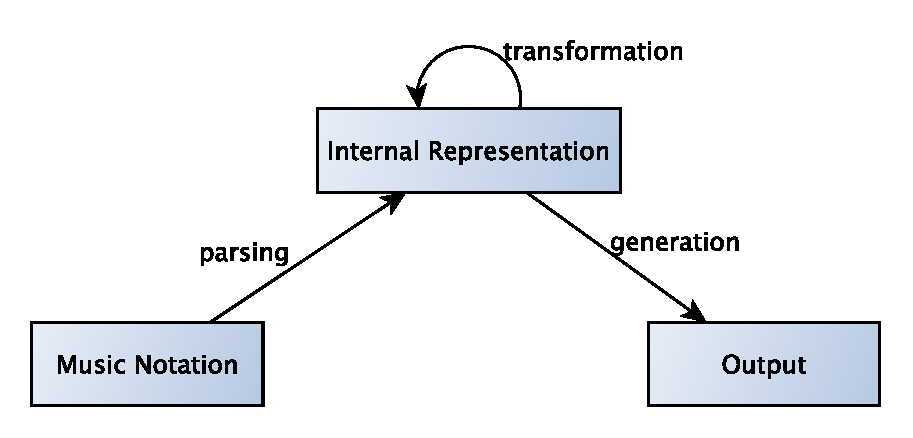
\includegraphics[width=0.8\textwidth]{img/proof_of_concept_general.pdf} 
  \caption{Process stages}
  \label{fig:process_stages}
\end{figure}

\subsection{Data Extraction} 

As written in subsection \ref{sec:abcm2ps_approach} the parser from abcm2ps will be used as well as
the internal representation that it generates. Next an analysis of both will be made.

\subsubsection{Abc Parser} 

The parser that is required for the extraction of abc data has to be robust, i.e., be able to expect
cases that it doesn't recognize and above all it has to be the cheapest possible in terms of time
wasted on its construction.

The solutions encountered to build the parser were three: to build one from scratch; to pick one
existing parser from programs like abcm2ps, abc2midi and try to adapt it to the requirements; and
use one of those existing parsers.\\
As the cost of building a parser was an essential requirement, the first two solutions were
discarded and the last one remained. So abcm2ps's parser was the natural choice for the reasons
described in subsection \ref{sec:abcm2ps_approach}.

\subsubsection{Internal Representation Adaptation}

A generic structure of the generated representation was modeled and it can be consulted in appendix
\ref{sec:generic_structure_of_abcm2ps_parser_internal_representation}.

The parser from abcm2ps is implemented in C so the generated structure had to be adapted to an
equivalent structure in order that scripting could be applied on it, more specifically in the 
language Perl.\\
So a little program was made in the language C that parses an Abc file then traverses the generated
structure and prints to the output the adapted structure. Subsequently the printed output is
evaluated to a Perl structure. The latter represents a Perl hash that maps the original structure.
It has the benefit of enabling Perl to easily evaluate and process it.\\
In the next stage a generic processor, which will be described in the next section, uses the adapted
structure to apply some transformations.\\

Figure \ref{fig:data_extraction} depicts the internal workflow of the Data Extraction stage. The
program described in this subsection is represented by the box 'C2Perl'.

\begin{figure}[htb]
  \centering 
  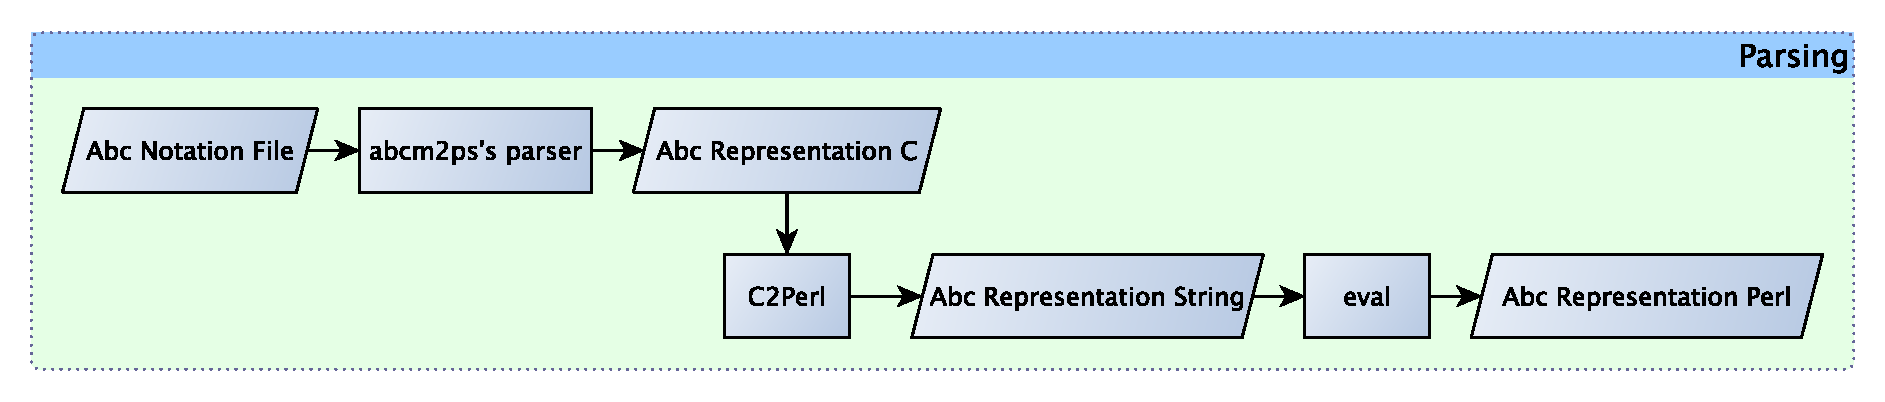
\includegraphics[width=\textwidth]{img/proof_of_concept_data_extrct.pdf} 
  \caption{Data Extraction}
  \label{fig:data_extraction}
\end{figure}

\subsection{Transformation of the generated representation}

At this stage the Unix philosophy had to be applied. However, programs like cut and paste were too
complex to implement without any kind of common process. So, to save the effort that implementing
such elaborate programs would take, a preliminary scripting was made.

This preliminary scripting consists of a generic processor that allows doing many tasks at once
instead of just one.\\
The requirements for this processor are:
\begin{description}
  \item[Higher-Order Processing] \hfill \\
    It must take as input one or more functions specified by the user and an Abc file (which will
    become the internal representation). And return a transformed structure, in which the functions
    passed in were applied to the structure's symbols.
  \item[Systematic] \hfill \\
    It has to be as systematic as possible, meaning that the specification of a function and the
    symbol it will be applied to has to be well defined.
  \item[Set of processing strategies defined] \hfill \\
    There must be a table of strategies where each strategy defines how the results of processing a
    symbol are to be merged with the others. 
\end{description}

\subsubsection{Processor Algorithm}

The internal representation processing is guided by its structure, meaning that it is applied to
each symbol.\\
The processor comprises a set of functions that define how each symbol should be processed
according to its internal values. Additionally it can use a function -default that is applied to a
symbol if no function is specified for it.\\
Moreover if neither is defined a default function is applied, this is the identity function, in
other words, it returns the original Abc of the symbol.\\
Optionally a -end function can be defined. It is used to allow storing in the processor a function
that executes a post processing of the obtained result. Thus attaining different output formats.

To ensure the system is systematic and compact, each function should be able to access global
variables like the current onset of the score or the current voice for each symbol. Those variables
grant a more complete control of what can be processed.

In order to define how the results of processing a symbol should be merged with others, the
processor must know which processing strategy it must use. Thus a table of strategies is needed and
by default the processor uses the STR strategy which makes the concatenation of the results of each
symbol.\\
Other strategies might be added to the table. For instance, a strategy that maps a set of symbols to
a Perl structure so that it can be processed as whole. Such a set might be difficult to process with
the default strategy.

This algorithm was inspired in the one used in XML::DT\cite{tesejj}, a processing module of XML
documents written by José João Dias.
%TODO procurar artigos Estratego

\subsection{Output Generation}
In this stage the transformed representation is outputted and it may be of the same type as the
input, which allows the articulation of different programs.


\section{Example}
In this section an academic example will be presented so that the usage of this general processor
might be better understood.

In Wiki::Score transcriptions, when there is more than one voice in a score and one of them ends
before all others because it has no more music, it's a known habit that transcribers do not fill the
remaining measures\footnote{The terminology being used here agrees to the one used in American
  English, i.e., the word 'bar' refers to the vertical line and the word 'measure' refers to the beats
contained between bars.} with rests. Knowing this it would be expected that a program should
automatically fill those empty measures. A way to accomplish this would be to count the number of
measures per voice and from that knowledge determine in which voices rests should be appended.

So the process for counting measures corresponds to a simple counting of bars, therefore it
will consist of mapping to the bar symbol a function that increments a counter for each voice
everytime a bar is found. The output generated, in other words, the -end function, will become the
writing of the counter's final values.\\

The code for this example is presented next.

% \abcinput{../ABC/corpus/fuga_bwv_578_excerpt.abc}

\lstinputlisting[language=Perl]{../ABC/tools/count_measures.pl}

In line 6, the function being called 'processor' corresponds to the general processor this proof of
concept has been describing.\\
In line 9, an association is made between the symbol that represents a bar and the function that
does the counting. Note that \$voice is a global variable that is assigned by the processor during
its traverse of the structure. It indicates the current voice being processed.\\
In line 10, the post processing function is defined, in other words, the measure counters are
printed for each voice.\\

The output for this program could be:
\lstset{numbers=none}
\begin{lstlisting}
Soprano has 21 bar(s).
Alto has 20 bar(s).
Tenor has 21 bar(s).
Bass has 21 bar(s).
\end{lstlisting}

The number of bars for the voice 'Alto' is different from the others. This means that an anomaly may
exist in the score. Then the user could, for instance, manually fix the problem in the actual score.

\section{Summary}

This proof of concept demonstrates that with a not so complicated algorithm, it is possible to
process, transform and generate Abc documents, along with statistics in a simple way. Additionally
it allows the articulation of independent utilizations of this algorithm.

Hereupon, the final goal doesn't seem so far away as it initially did. The philosophy of tackling
the parts of a whole so that the actual problem can be solved in a less complicated way helps
reducing the complexity of building such elaborate tools as a Unix \textit{cut} for Abc files.\\

\end{document}
